\section{Riemann Sums} \label{S:4.2.Riemann}

\begin{goals}
\item How can we use a Riemann sum to estimate the area between a given curve and the horizontal axis over a particular interval?

\item What are the differences among left, right, middle, and random Riemann sums?

\item What is sigma notation and how does this enable us to write Riemann sums in an abbreviated form?
\end{goals}

%----------------------------------
% SUBSECTION INTRODUCTION
%----------------------------------
\subsection*{Introduction}

\begin{marginfigure}[3in] % MARGIN FIGURE
\margingraphics{figs/4/4-2_Intro.pdf}
\caption{A velocity function that is sometimes negative.} \label{fig:4.2_Intro}
\end{marginfigure}

In Section~\ref{S:4.1.VelocityDistance}, we learned that if we have a moving object with velocity function $v$, whenever $v(t)$ is positive, the area between $y = v(t)$ and the $t$-axis over a given time interval tells us the distance traveled by the object over that time period; in addition, if $v(t)$ is sometimes negative and we view the area of any region below the $t$-axis as having an associated negative sign, then the sum of these signed areas over a given interval tells us the moving object's change in position over the time interval.

For instance, for the velocity function given in Figure~\ref{fig:4.2_Intro}, if the areas of shaded regions are $A_1$, $A_2$, and $A_3$ as labeled, then the total distance $D$ traveled by the moving object on $[a,b]$ is 
\[ D = A_1 + A_2 + A_3, \]
while the total change in the object's position on $[a,b]$ is 
\[ s(b) - s(a) = A_1 - A_2 + A_3. \]
Because the motion is in the negative direction on the interval where $v(t) < 0$, we subtract $A_2$ when determining the object's total change in position.

Of course, finding $D$ and $s(b)-s(a)$ for the situation given in Figure~\ref{fig:4.2_Intro} presumes that we can actually find the areas represented by $A_1$, $A_2$, and $A_3$.  In most of our work in Section~\ref{S:4.1.VelocityDistance}, such as in Activities~\ref{A:4.1.2} and~\ref{A:4.1.3}, we worked with velocity functions that were either constant or linear, so that by finding the areas of rectangles and triangles, we could find the area bounded by the velocity function and the horizontal axis exactly.  But when the curve that bounds a region is not one for which we have a known formula for area, we are unable to find this area exactly.  Indeed, this is one of our biggest goals in Chapter~\ref{CH:4}: to learn how to find the exact area bounded between a curve and the horizontal axis for as many different types of functions as possible.  

To begin, we expand on the ideas in Activity~\ref{A:4.1.1}, where we encountered a nonlinear velocity function and approximated the area under the curve using four and eight rectangles, respectively.  In the following preview activity, we focus on three different options for deciding how to find the heights of the rectangles we will use.

\begin{marginfigure}[2cm] % MARGIN FIGURE
\captionsetup[subfigure]{labelformat=empty}
\begin{center}
\subfloat{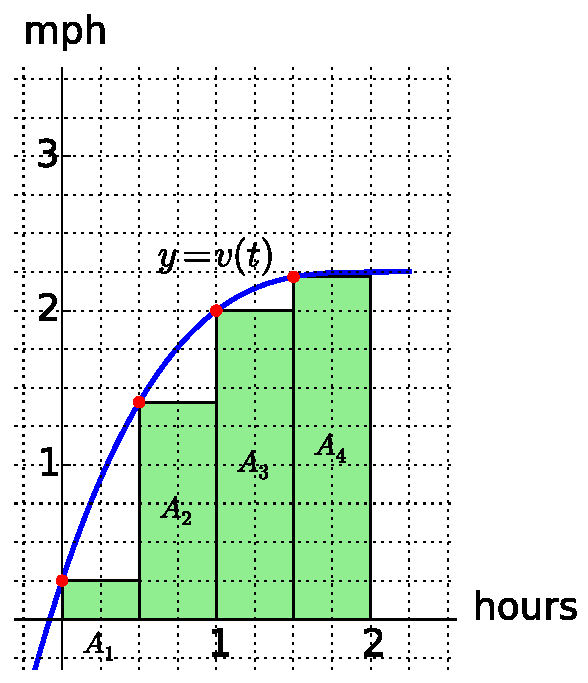
\includegraphics[scale=.5]{figs/4/preview_4-2a.pdf}}

\subfloat{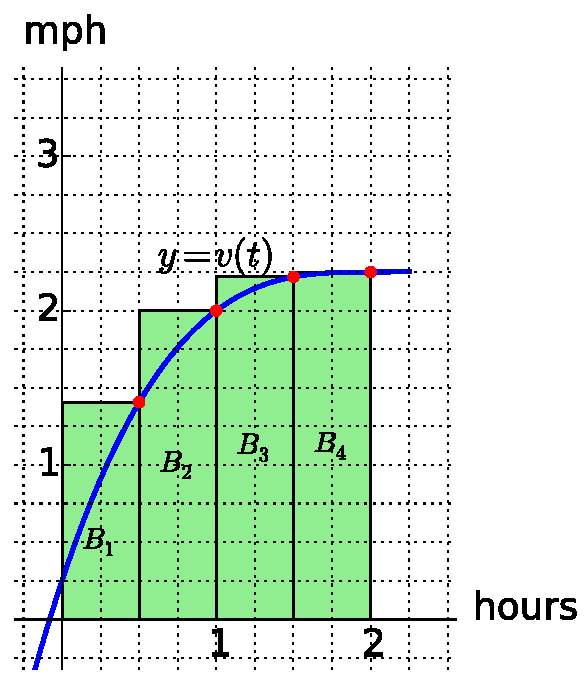
\includegraphics[scale=.5]{figs/4/preview_4-2b.pdf}}

\subfloat{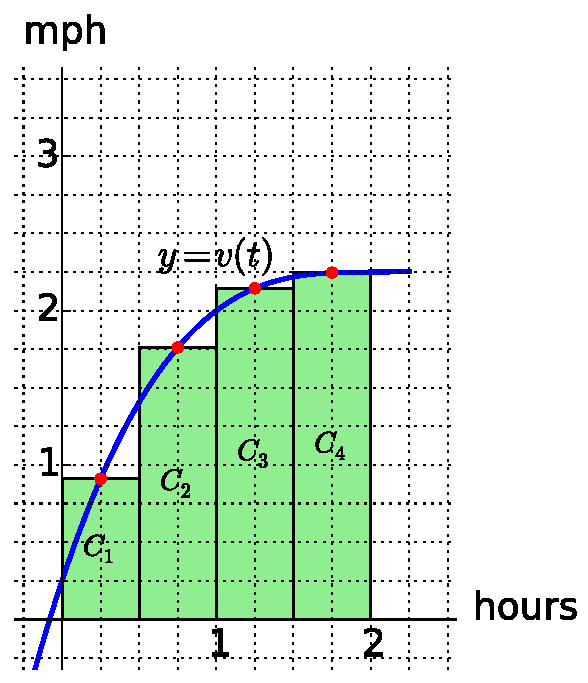
\includegraphics[scale=.5]{figs/4/preview_4-2c.pdf}}
\caption{Estimating the area under $y = v(t)$.} \label{fig:4.2.PA1}
\end{center}
\end{marginfigure}

%\begin{marginfigure} % MARGIN FIGURE
%\captionsetup[subfigure]{labelformat=empty}
%\subfloat{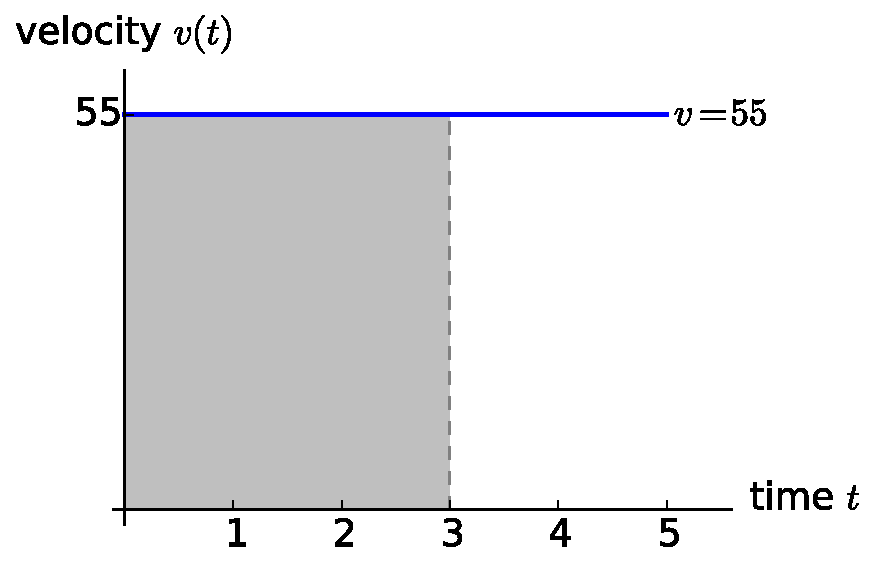
\includegraphics[width=\marginparwidth]{figs/0/position_t3.pdf}}
%
%\subfloat{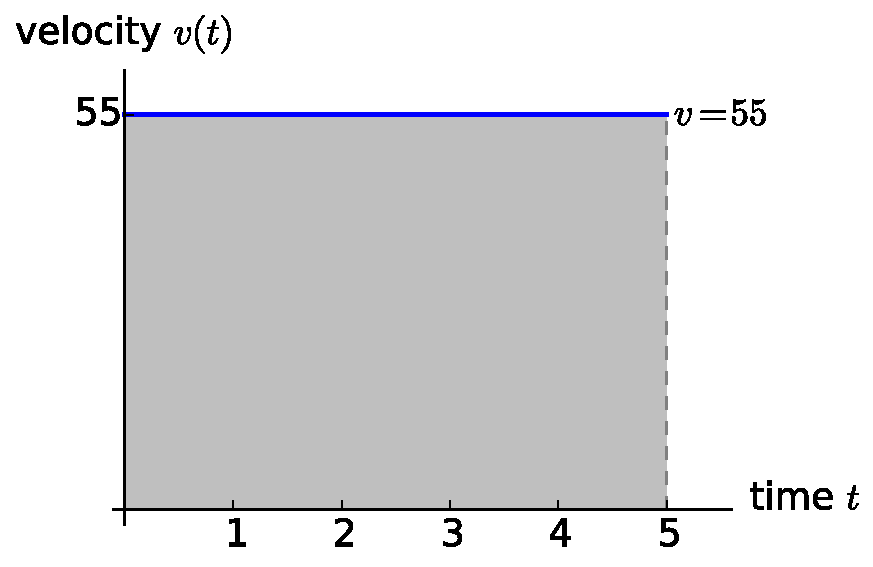
\includegraphics[width=\marginparwidth]{figs/0/position_t5.pdf}}
%\caption{Position at $t=3$ and $t=5$ represented by the area of a rectangle.}
%\label{fig:0-position_t5}
%\end{marginfigure}

\begin{pa} \label{PA:4.2}
A person walking along a straight path has her velocity in miles per hour at time $t$ given by the function $v(t) = 0.25t^3-1.5t^2+3t+0.25$, for times in the interval $0 \le t \le 2$.  The graph of this function is also given in each of the three diagrams. Note that in each diagram, we use four rectangles to estimate the area under $y = v(t)$ on the interval $[0,2]$, but the method by which the four rectangles' respective heights are decided varies among the three individual graphs.
\ba
\item How are the heights of rectangles in the left-most diagram being chosen?  Explain, and hence determine the value of 
\[ S = A_1 + A_2 + A_3 + A_4 \]
by evaluating the function $y = v(t)$ at appropriately chosen values and observing the width of each rectangle.  Note, for example, that 
\[ A_3 = v(1) \cdot \frac{1}{2} = 2 \cdot \frac{1}{2} = 1. \]

\item Explain how the heights of rectangles are being chosen in the middle diagram and find the value of
\[ T = B_1 + B_2 + B_3 + B_4. \]

\item Likewise, determine the pattern of how heights of rectangles are chosen in the right-most diagram and determine
\[ U = C_1 + C_2 + C_3 + C_4. \]
	
\item Of the estimates $S$, $T$, and $U$, which do you think is the best approximation of $D$, the total distance the person traveled on $[0,2]$?  Why?
\ea
\end{pa} 
\afterpa % PREVIEW ACTIVITY

%-------------------------------------
% SUBSECTION SIGMA NOTATION
%-------------------------------------
\subsection*{Sigma Notation}

It is apparent from several different problems that sums of areas of rectangles is one of the main ways to approximate the area under a curve over a given interval.  Intuitively, we expect that using a larger number of thinner rectangles will provide a way to improve the estimates we are computing.  As such, we anticipate dealing with sums with a large number of terms.  To do so, we introduce the use of so-called \emph{sigma notation}\index{sigma notation}, named for the Greek letter $\Sigma$, which is the capital letter $S$ in the Greek alphabet.

For example, say we are interested in the sum
\[ 1 + 2 + 3 + \cdots + 100, \]
which is the sum of the first $100$ natural numbers.  Sigma notation provides a shorthand notation that recognizes the general pattern in the terms of the sum.  It is equivalent to write
\[ \sum_{k=1}^{100} k =  1 + 2 + 3 + \cdots + 100. \]
We read the symbol $\ds \sum_{k=1}^{100} k$ as ``the sum from $k$ equals $1$ to $100$ of $k$.''  The variable $k$ is usually called the index of summation, and the letter that is used for this variable is immaterial.  

Suppose we wish to add up a list of numbers $a_1$, $a_2$, $a_3$, \ldots, $a_9$. Instead of writing $\ds a_1+a_2+a_3+a_4+a_5+a_6+a_7+a_8+a_9,$
we use sigma notation and write 
\[ \sum_{i=1}^9 a_i. \]
Again, the capital sigma represents the term ``sum.'' The index of summation in this example is $i$. By convention, the index takes on only the integer values between (and including) the lower and upper bounds. 

Each summand in sigma notation involves a function of the index; for example,
\begin{eqnarray*}
\sum_{k=1}^{10} (k^2 + 2k) & = & (1^2 + 2\cdot 1) + (2^2 + 2\cdot 2) + (3^2 + 2\cdot 3) \\
& & + \cdots + (10^2 + 2\cdot 10),
\end{eqnarray*}
and more generally,
$$\sum_{k=1}^n f(k) = f(1) + f(2) + \cdots + f(n).$$
Sigma notation allows us the flexibility to easily vary the function being used to track the pattern in the sum, as well as to adjust the number of terms in the sum simply by changing the value of $n$.  We test our understanding of this new notation in the following activity.

\begin{activity} \label{A:4.2.1}  For each sum written in sigma notation, write the sum long-hand and evaluate the sum to find its value.  For each sum written in expanded form, write the sum in sigma notation.
\ba
	\item $\ds \sum_{k=1}^{5} (k^2 + 2)$
	\item $\ds \sum_{i=3}^{6} (2i-1)$
	\item $\ds 3 + 7 + 11 + 15 +  \cdots + 27$
	\item $\ds 4 + 8 + 16 + 32 \cdots + 256$
	\item $\ds \sum_{i=1}^{6} \frac{1}{2^i}$
\ea
\end{activity}
\begin{smallhint}
\ba
	\item Observe that when $k = 1$, $k^2 + 2 = 1^2 + 2 = 3$.  This is the first term in the sum.
	\item Note that this sum starts at $i = 3$.
	\item Since the terms in the sum increase by 4, try a function $f(k)$ that somehow involves $4k$.
	\item What pattern do you observe in the terms of the sum?
	\item Write every term in the sum as a fraction with denominator $2^6 = 64$.
\ea
\end{smallhint}
\begin{bighint}
\ba
	\item Observe that when $k = 1$, $k^2 + 2 = 1^2 + 2 = 3$.  This is the first term in the sum.  The last term in the sum occurs when $k = 5$, which is $5^2 + 2 = 27$.
	\item Note that this sum starts at $i = 3$ and the first term is $(2\cdot 3 - 1) = 5$.
	\item Since the terms in the sum increase by 4, try a function $f(k)$ that somehow involves $4k$.  You have freedom to decide where your index $k$ starts; try $k = 1$.
	\item What pattern do you observe in the terms of the sum?
	\item Write every term in the sum as a fraction with denominator $2^6 = 64$.
\ea
\end{bighint}
\begin{activitySolution}
\ba
	\item 
	\begin{eqnarray*}
	 \sum_{k=1}^{5} (k^2 + 2) & = & (1^2 + 2) + (2^2 + 2) + (3^2 + 2) + (4^2 + 2) + (5^2 + 2) \\
	 					& = & 3 + 6 + 11 + 17 + 27 \\
						& = & 64
	\end{eqnarray*}
	\item 
	\begin{eqnarray*}
	 \sum_{i=3}^{6} (2i-1) & = & (2 \cdot 3 - 1) + (2 \cdot 4- 1) + (2 \cdot 5 - 1) + (2 \cdot 6 - 1) \\
	 				& = & 5 + 7 + 9 + 11 \\
					& = & 32
	\end{eqnarray*}
	\item Observe that each term in the sum
	$$\ds 3 + 7 + 11 + 15 +  \cdots + 27$$
	differs from the previous term by 4.  If we view $4$ as $4 = 4 \cdot 1 - 1$ and $7$ as $7 = 4 \cdot 2 - 1$, we see that the pattern may be represented through the function $f(k) = 4k-1$, so that
	$$\ds 3 + 7 + 11 + 15 +  \cdots + 27 = \sum_{k=1}^{7} 4k-1.$$
	We note that $k=7$ is the end value of the index since $4 \cdot 7  = 28$.
	\item The sum $\ds 4 + 8 + 16 + 32 + \cdots + 256$ is a sum of powers of $2$, which we can express in sigma notation as
	$$4 + 8 + 16 + 32 + \cdots + 256 = \sum{i=2}^{8} 2^i.$$
	\item
	\begin{eqnarray*}
	  \sum_{i=1}^{6} \frac{1}{2^i} & = & \frac{1}{2} + \frac{1}{2^2} + \cdots + \frac{1}{2^6} \\
	  					& = & \frac{32}{64} + \frac{16}{64} + \frac{8}{64} + \frac{4}{64} + \frac{2}{64} + \frac{1}{64} \\
						& = & \frac{63}{64}.
	\end{eqnarray*}
\ea
\end{activitySolution}
\aftera % ACTIVITY

It might seem odd to stress a new, concise way of writing summations only to write each term out as we add them up. It is. Therefore, we give some properties of summations that allow us to work with them without writing individual terms. 

\definition{Properties of Summations\index{summation!properties}} % DEFINITION
{
\begin{enumerate}[1)]
\item	$\ds \sum_{i=1}^n c = c\cdot n$, where $c$ is a constant.
\item	$\ds \sum_{i=1}^n c\cdot a_i = c\cdot\sum_{i=1}^n a_i$
\item	$\ds \sum_{i=m}^n (a_i\pm b_i) = \sum_{i=m}^n a_i \pm \sum_{i=m}^n b_i$
\end{enumerate}
\begin{multicols}{2}
\begin{enumerate}[1),resume]
\item	$\ds \sum_{i=m}^j a_i + \sum_{i=j+1}^n  a_i = \sum_{i=m}^n a_i$
\item	$\ds \sum_{i=1}^n i = \frac{n(n+1)}2$
\item	$\ds \sum_{i=1}^n i^2 = \frac{n(n+1)(2n+1)}6$
\item	$\ds \sum_{i=1}^n i^3 = \left(\frac{n(n+1)}2\right)^2$
\end{enumerate}
\end{multicols}
$\left.\right.$
} % end definition

\begin{example} % EXAMPLE
Evaluate $\ds  \sum_{i=1}^6 (2i-1)$. 

\solution 
\begin{align*}
\sum_{i=1}^6 (2i-1) & = \sum_{i=1}^6 2i - \sum_{i=1}^6 1 \\
& = 2\sum_{i=1}^6 i - \sum_{i=1}^6 1 \\
& = 2 \left( \frac{6(6+1)}{2} \right) - 6 \\
& = 42-6 \\
& = 36
\end{align*}
We obtained the same answer without writing out all six terms. When dealing with small sizes of $n$, it may be faster to write the terms out by hand. However, the Properties of Summations are incredibly important when dealing with large sums as we'll soon see.
\end{example} % EXAMPLE 

%-------------------------------------
% SUBSECTION RIEMANN SUMS
%-------------------------------------
\subsection*{Riemann Sums}

When a moving body has a positive velocity function $y = v(t)$ on a given interval $[a,b]$, we know that the area under the curve over the interval is the total distance the body travels on $[a,b]$.  While this is the fundamental motivating force behind our interest in the area bounded by a function, we are also interested more generally in being able to find the exact area bounded by $y = f(x)$ on an interval $[a,b]$, regardless of the meaning or context of the function $f$.  For now, we continue to focus on determining an accurate estimate of this area through the use of a sum of the areas of rectangles, doing so in the setting where $f(x) \ge 0$ on $[a,b]$.  Throughout, unless otherwise indicated, we also assume that $f$ is continuous on $[a,b]$.

The first choice we make in any such approximation is the number of rectangles.  If we say that the total number of rectangles is $n$, and we desire $n$ rectangles of equal width to subdivide the interval $[a,b]$, then each rectangle must have width $\triangle x = \frac{b-a}{n}$. We observe further that $x_1 = x_0 + \triangle x$, $x_2 = x_0 + 2 \triangle x$, and thus in general $x_{i} = a + i\triangle x,$ as pictured in Figure~\ref{fig:4-2_Interval}.

\begin{marginfigure} % MARGIN FIGURE
\margingraphics{figs/4/4-2_Interval.pdf}
\caption{Subdividing the interval $[a,b]$ into $n$ subintervals of equal length $\Delta x$.} \label{fig:4-2_Interval}
\end{marginfigure}

We use each subinterval $[x_i, x_{i+1}]$ as the base of a rectangle, and next must choose how to decide the height of the rectangle that will be used to approximate the area under $y = f(x)$ on the subinterval.  There are three standard choices:  use the left endpoint of each subinterval, the right endpoint of each subinterval, or the midpoint of each.  These are precisely the options encountered in Preview Activity~\ref{PA:4.2} and seen in Figure~\ref{fig:4.2.PA1}.  We next explore how these choices can be reflected in sigma notation.

If we now consider an arbitrary positive function $f$ on $[a,b]$ with the interval subdivided as shown in Figure~\ref{fig:4-2_Interval}, and choose to use left endpoints, then on each interval of the form $[x_{i}, x_{i+1}]$, the area of the rectangle formed is given by
\[ A_{i+1} = f(x_i) \cdot \triangle x,\]
as seen in Figure~\ref{fig:4.2_LeftSum}.

\begin{marginfigure} % MARGIN FIGURE
\margingraphics{figs/4/4-2_LeftSum.pdf}
\caption{Subdividing the interval $[a,b]$ into $n$ subintervals of equal length $\triangle x$ and approximating the area under $y = f(x)$ over $[a,b]$ using left rectangles.} \label{fig:4.2_LeftSum}
\end{marginfigure}

If we let $L_n$ denote the sum of the areas of rectangles whose heights are given by the function value at each respective left endpoint, then we see that
\begin{eqnarray*}
L_n & = & A_1 + A_2 + \cdots + A_{i+1} + \cdots + A_n \\
	& = & f(x_0) \cdot \triangle x + f(x_1) \cdot \triangle x + \cdots + f(x_i) \cdot \triangle x \\ 
& & + \cdots + f(x_{n-1}) \cdot \triangle x.
\end{eqnarray*}
In the more compact sigma notation, we have 
\[ L_n = \sum_{i = 0}^{n-1} f(x_i) \triangle x. \]
Note particularly that since the index of summation begins at $0$ and ends at $n-1$, there are indeed $n$ terms in this sum.  We call $L_n$ the \emph{left Riemann sum} \index{Riemann sum} \index{Riemann sum!left} for the function $f$ on the interval $[a,b]$.

\begin{marginfigure}[3in] % MARGIN FIGURE
\margingraphics{figures/4_2_RenaultAppletRS.pdf}
\caption{A snapshot of the applet found at \href{http://gvsu.edu/s/a9}{\texttt{http://gvsu.edu/s/a9}}.} \label{F:4.2.RenaultAppletRS}
\end{marginfigure}

There are now two fundamental issues to explore:  the number of rectangles we choose to use and the selection of the pattern by which we identify the height of each rectangle.  It is best to explore these choices dynamically, and the applet found at \href{http://gvsu.edu/s/a9}{\texttt{http://gvsu.edu/s/a9}} is a particularly useful one.  There we see the image shown in Figure~\ref{F:4.2.RenaultAppletRS}, but with the opportunity to adjust the slider bars for the left endpoint and the number of subintervals.  By moving the sliders, we can see how the heights of the rectangles change as we consider left endpoints, midpoints, and right endpoints, as well as the impact that a larger number of narrower rectangles has on the approximation of the exact area bounded by the function and the horizontal axis.  

To see how the Riemann sums for right endpoints and midpoints are constructed, we consider Figure~\ref{fig:4-2_RightSum} and Figure~\ref{fig:4-2_MidSum}. For the sum with right endpoints, we see that the area of the rectangle on an arbitrary interval $[x_i, x_{i+1}]$ is given by
\[ B_{i+1} = f(x_{i+1}) \cdot \triangle x, \]
so that the sum of all such areas of rectangles is given by
\begin{eqnarray*}
R_n & = & B_1 + B_2 + \cdots + B_{i+1} + \cdots + B_n \\
& = &  f(x_1) \cdot \triangle x + f(x_2) \cdot \triangle x + \cdots + f(x_{i+1}) \cdot \triangle x \\
& & + \cdots + f(x_{n}) \cdot \triangle x \\ 
& = & \sum_{i=1}^{n} f(x_i) \triangle x.
\end{eqnarray*}
We call $R_n$ the \emph{right Riemann sum} \index{Riemann sum!right} for the function $f$ on the interval $[a,b]$.  

For the sum that uses midpoints, we introduce the notation
\[ \overline{x}_{i+1} = \frac{x_{i} + x_{i+1}}{2} \]
so that $\overline{x}_{i+1}$ is the midpoint of the interval $[x_i, x_{i+1}]$.  For instance, for the rectangle with area $C_1$ in Figure~\ref{fig:4-2_MidSum}, we now have
\[ C_1 = f(\overline{x}_1) \cdot \triangle x. \]

\begin{marginfigure}[-7cm] % MARGIN FIGURE
\margingraphics{figs/4/4-2_RightSum.pdf}
\caption{Riemann sums using right endpoints.} \label{fig:4-2_RightSum}
\end{marginfigure}

\begin{marginfigure} % MARGIN FIGURE
\margingraphics{figs/4/4-2_MidSum.pdf}
\caption{Riemann sums using midpoints.} \label{fig:4-2_MidSum}
\end{marginfigure}

Hence, the sum of all the areas of rectangles that use midpoints is 
\begin{eqnarray*}
M_n & = & C_1 + C_2 + \cdots + C_{i+1} + \cdots + C_n \\
& = &  f(\overline{x_1}) \cdot \triangle x + f(\overline{x_2}) \cdot \triangle x + \cdots + f(\overline{x}_{i+1}) \cdot \triangle x \\
& & + \cdots + f(\overline{x}_{n}) \cdot \triangle x \\ 
& = & \sum_{i=1}^{n} f(\overline{x}_i) \triangle x,
\end{eqnarray*}
and we say that $M_n$ is the \emph{middle Riemann sum} \index{Riemann sum!middle} for $f$ on $[a,b]$.

\begin{example} % EXAMPLE
Approximate the area of the region under $y=4x-x^2$ on the interval $[0,4]$ using $L_4$, $R_4$, and $M_4$. 

\solution We partition the interval $[0,4]$ into the four subintervals $[0,1]$, $[1,2]$, $[2,3]$, and $[3,4]$. In Figure~\ref{fig:apex_5-3_Area1}-(a) we see $4$ rectangles drawn on $f(x) = 4x-x^2$ using the $L_4$. Note how in the first subinterval, $[0,1]$, the rectangle has height $f(0)=0$. We add up the areas of each rectangle, which is width $\times$ height, for our $L_4$ approximation:
\begin{eqnarray*}
L_4 & = & 1 \cdot f(0) + 1 \cdot f(1)+ 1 \cdot f(2) + 1 \cdot f(3) \\
& = & 0+3+4+3 \\
& = & 10.
\end{eqnarray*}
	
Figure~\ref{fig:apex_5-3_Area1}-(b) shows $4$ rectangles drawn under $f$ using $R_4$; note how the rectangle on the subinterval $[3,4]$ has height $0$.  Our approximation gives the same answer as before, though calculated a different way:
\begin{eqnarray*}
R_4 & = & 1 \cdot f(1) + 1 \cdot f(2)+ 1 \cdot f(3) + 1 \cdot f(4) \\
& = & 3+4+3+0 \\
& = & 10.
\end{eqnarray*}

Figure~\ref{fig:apex_5-3_Area1}-(c) shows $4$ rectangles drawn under $f$ using $M_4$. Notice that the height of each of the rectangles is determined by the point in the middle of each subinterval, which are $0.5$, $1.5$, $2.5$, and $3.5$. So
\begin{eqnarray*}
M_4 & = & 1 \cdot f(0.5) + 1 \cdot f(1.5)+ 1 \cdot f(2.5) + 1 \cdot f(3.5) \\
& = & 1.75 + 3.75 + 3.75 + 1.75 \\
& = & 11.
\end{eqnarray*}
\end{example}

\begin{marginfigure} % MARGIN FIGURE
\begin{center}
%\captionsetup[subfigure]{labelformat=empty}
\subfloat[$L_n$]{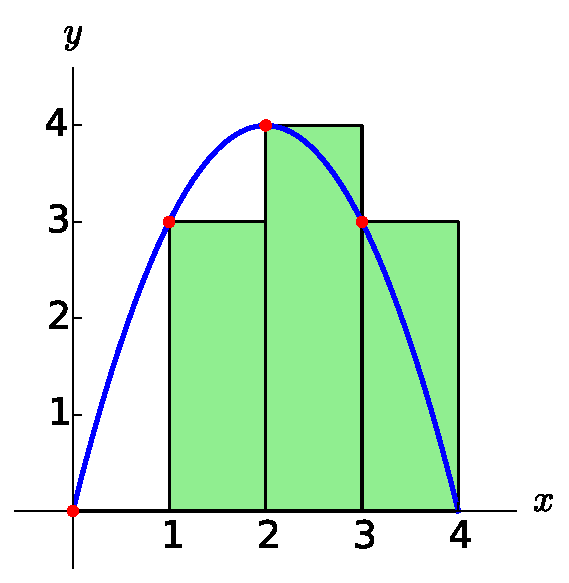
\includegraphics[scale=.5]{figs/4/apex_5-3_Area1Ln.pdf}}
%\caption{Approximating the area under $y=4x-x^2$ on $[0,4]$ using $L_n$} \label{fig:apex_5-3_Area1}

\subfloat[$R_n$]{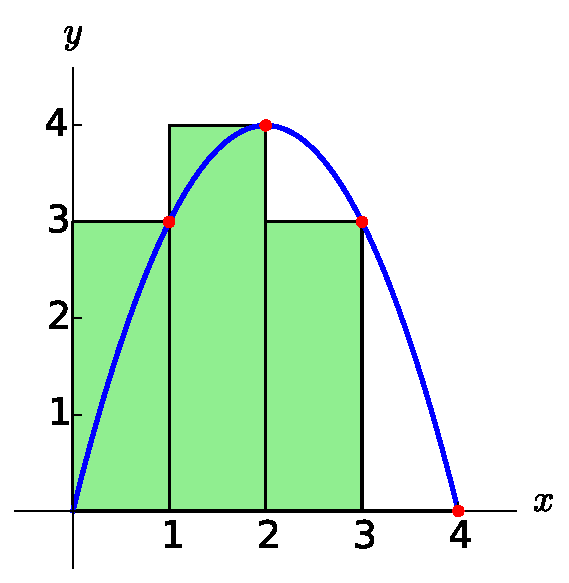
\includegraphics[scale=.5]{figs/4/apex_5-3_Area1Rn.pdf}}
%\caption{Approximating the area under $y=4x-x^2$ on $[0,4]$ using $R_n$} \label{fig:apex_5-3_Area1}

\subfloat[$M_n$]{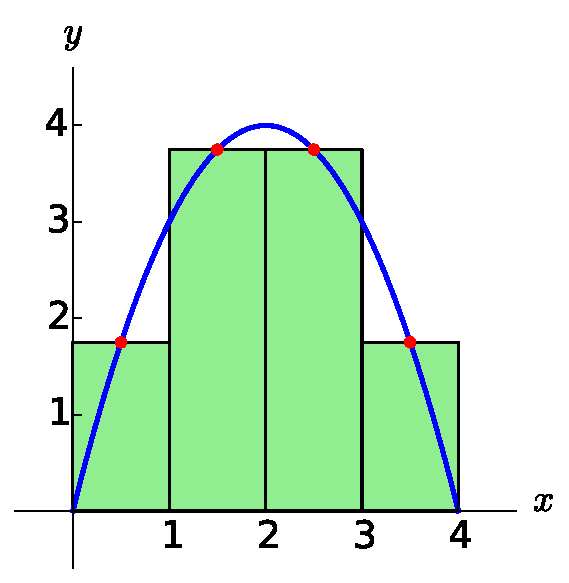
\includegraphics[scale=.5]{figs/4/apex_5-3_Area1Mn.pdf}}
\caption{Approximating the area under $y=4x-x^2$ on $[0,4]$ using $L_n$, $R_n$, and $M_n$} \label{fig:apex_5-3_Area1}
\end{center}
\end{marginfigure} % EXAMPLE

When $f(x) \ge 0$ on $[a,b]$, each of the Riemann sums $L_n$, $R_n$, and $M_n$ provides an estimate of the area under the curve $y = f(x)$ over the interval $[a,b]$; momentarily, we will discuss the meaning of Riemann sums in the setting when $f$ is sometimes negative.  We also recall that in the context of a nonnegative velocity function $y = v(t)$, the corresponding Riemann sums are approximating the distance traveled on $[a,b]$ by the moving object with velocity function $v$.

There is a more general way to think of Riemann sums, and that is to not restrict the choice of where the function is evaluated to determine the respective rectangle heights.  That is, rather than saying we'll always choose left endpoints, or always choose midpoints, we simply say that a point $x_{i+1}^*$ will be selected at random in the interval $[x_i, x_{i+1}]$ (so that $x_i \le x_{i+1}^* \le x_{i+1}$), which makes the Riemann sum given by
\begin{eqnarray*}
\ds \sum_{i=1}^{n} f(x_i^*) \triangle x & = & f(x_1^*) \cdot \triangle x + f(x_2^*) \cdot \triangle x + \cdots + f(x_{i+1}^*) \cdot \triangle x \\
& & + \cdots + f(x_n^*) \cdot \triangle x.
\end{eqnarray*}
At \href{http://gvsu.edu/s/a9}{\texttt{http://gvsu.edu/s/a9}}, the applet noted earlier and referenced in Figure~\ref{F:4.2.RenaultAppletRS}, by unchecking the ``relative'' box at the top left, and instead checking ``random,'' we can easily explore the effect of using random point locations in subintervals on a given Riemann sum.  In computational practice, we most often use $L_n$, $R_n$, or $M_n$, while the random Riemann sum is useful in theoretical discussions.  In the following activity, we investigate several different Riemann sums for a particular velocity function.

\begin{marginfigure}[8cm] % MARGIN FIGURE
\margingraphics{figs/4/apex_5-3_Area1Rn16.pdf}
\caption{Approximating the area under $y~=~4x-x^2$ on $[0,4]$ using $R_n$ with $n=16$.} \label{fig:apex_5-3_Area1Rn16}
\end{marginfigure}

\begin{example} % EXAMPLE
Approximate the area under $y=4x-x^2$ on $[0,4]$ using $R_n$ and summation formulas with $16$ and $1000$ equally spaced intervals.

\solution Using $16$ rectangles, we can approximate the area as 
\[ \sum_{i=1}^{16} f(x_i) \Delta x \]
where $\Delta x = 4/16 = 1/4$ and $x_i = 0 + i \Delta x = i \Delta x$. Using the properties of summations, we have
\begin{eqnarray}
\mbox{Area} & \approx & R_{16}  = \sum_{i=1}^{16} f(x_i) \Delta x \notag \\
&=& \sum_{i=1}^{16} f( i\Delta x ) \Delta x \notag \\
&=& \sum_{i=1}^{16} \left( 4i \Delta x - (i \Delta x)^2 \right) \Delta x \notag \\
&=& \sum_{i=1}^{16} \left( 4i \Delta x^2 - i^2 \Delta x^3 \right) \notag \\		
&=& \left( 4\Delta x^2 \right) \sum_{i=1}^{16} i - \left( \Delta x^3 \right) \sum_{i=1}^{16} i^2 \label{eq:rie7} \\ %\label{eq:rie7}
&=& (4\Delta x^2)\frac{16\cdot 17}{2} - \left( \Delta x^3 \right) \frac{16(17)(33)}6 \notag \\
&=&	4 \cdot \left( \frac{1}{4} \right)^2 \cdot \frac{16\cdot 17}{2} - \left( \frac{1}{4} \right)^3 \cdot \frac{16(17)(33)}{6} \notag \\
&=&	2 \cdot 17 - \frac{17 \cdot 11}{8} \notag \\
&=& \frac{85}{8} = 10.625 \notag
\end{eqnarray}
We were able to sum up the areas of $16$ rectangles with very little computation. Notice  Equation \eqref{eq:rie7}; by changing the $16$'s to $1,000$'s (and appropriately changing the value of $\Delta x$ to $4/1000$), we can use that equation to sum up $1000$ rectangles!
\begin{align*}
\mbox{Area} & \approx R_{1000} = \sum_{i=1}^{1000} f(x_i) \Delta x \\
&= \left( 4 \Delta x^2 \right) \sum_{i=1}^{1000} i - \left(\Delta x^3 \right) \sum_{i=1}^{1000} i^2 \\
&= \left( 4 \Delta x^2 \right) \frac{1000 \cdot 1001}{2} - \left( \Delta x^3 \right) \frac{1000(1001)(2001)}6 \\
&= 4 \cdot (0.004)^2 \cdot 500500 - (0.004)^3\cdot 333,833,500\\
&= 10.666656
\end{align*}

Using this many rectangles, it's likely that we have a good approximation of the area under $y=4x-x^2$ on $[0,4]$. That is, the area is approximately $10.666656$.
\end{example} % EXAMPLE

\begin{activity} \label{A:4.2.2}  Suppose that an object moving along a straight line path has its velocity in feet per second at time $t$ in seconds given by $\ds v(t) = \frac{2}{9}(t-3)^2 + 2$.
\ba
\item Carefully sketch the region whose exact area will tell you the value of the distance the object traveled on the time interval $2 \le t \le 5$.
	
\item Estimate the distance traveled on $[2,5]$ by computing $L_4$, $R_4$, and $M_4$.

\item Does averaging $L_4$ and $R_4$ result in the same value as $M_4$?  If not, what do you think the average of $L_4$ and $R_4$ measures?

\item For this question, think about an arbitrary function $f$, rather than the particular function $v$ given above.  If $f$ is positive and increasing on $[a,b]$, will $L_n$ over-estimate or under-estimate the exact area under $f$ on $[a,b]$?  Will $R_n$ over- or under-estimate the exact area under $f$ on $[a,b]$? Explain.
\ea
\end{activity}

\begin{smallhint}
\ba
	\item Note that $y = v(t)$ is a parabola with vertex $(3,2)$.
	\item Recall the formulas for $L_n$, $R_n$, and $M_n$.
	\item Think about what the average of $L_1$ and $R_1$ measures.
	\item Consider carefully the role of endpoints in generating $L_n$ and $R_n$.
\ea
\end{smallhint}
\begin{bighint}
\ba
	\item Note that $y = v(t)$ is a parabola with vertex $(3,2)$.
	\item Recall the formulas for $L_n$, $R_n$, and $M_n$.
	\item Think about what the average of $L_1$ and $R_1$ measures.
	\item Consider carefully the role of endpoints in generating $L_n$ and $R_n$ and what you know about the behavior of an always increasing function.
\ea
\end{bighint}
\begin{activitySolution}
\ba
	\item The region whose exact area tells us the value of the distance the object traveled on the time interval $2 \le t \le 5$ is shown below.
	\begin{center}
		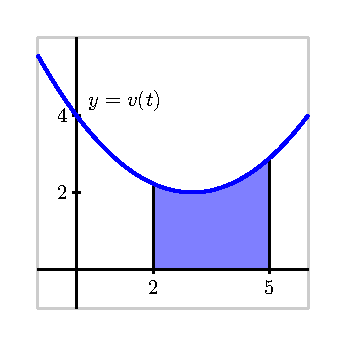
\includegraphics{figures/4_2_Act2Soln.eps}
	\end{center}
	\item $L_4 = \frac{311}{48} \approx 6.47917$, 
	        $R_4 = \frac{335}{48} \approx 6.97917$, and 
	        $M_4 = \frac{637}{96} \approx 6.63542$.
	\item The average of $L_4$ and $R_4$ is
	$$\frac{L_4 + M_4}{2} = \frac{311+335}{96} = \frac{646}{96} \ne \frac{637}{96} = M_4.$$
	This average actually measures what would result from using four trapezoids, rather than rectangles, to estimate the area on each subinterval.  One reason this is so is because the area of a trapezoid is the average of the bases times the width, and the ``bases'' are given by the function values at the left and right endpoints.
	\item If $f$ is positive and increasing on $[a,b]$, $L_n$ will under-estimate the exact area under $f$ on $[a,b]$.  Because $f$ is increasing, its value at the left endpoint of any subinterval will be lower than every other function value in the interval, and thus the rectangle with that height lies exclusively below the curve.  In a similar way, $R_n$ over-estimates the exact area under $f$ on $[a,b]$.
\ea
\end{activitySolution}
\aftera % ACTIVITY

%------------------------------------------------------------------------
% SUBSECTION WHEN THE FUNCTION IS SOMETIMES NEGATIVE
%------------------------------------------------------------------------
\subsection*{When the function is sometimes negative}

For a Riemann sum such as 
$$L_n = \sum_{i=0}^{n-1} f(x_i) \triangle x,$$
we can of course compute the sum even when $f$ takes on negative values.  We know that when $f$ is positive on $[a,b]$, the corresponding left Riemann sum $L_n$ estimates the area bounded by $f$ and the horizontal axis over the interval.

\begin{marginfigure}[-5cm] % MARGIN FIGURE
\margingraphics{figs/4/4-2_NegFa.pdf}
\caption{A left Riemann sum for a function $f$ that is sometimes negative.} \label{fig:4-2_NegFa}
\end{marginfigure}

For a function such as the one pictured in Figure~\ref{fig:4-2_NegFa}, where in the figure a left Riemann sum is being taken with $12$ subintervals over $[a,d]$, we observe that the function is negative on the interval $b \le x \le c$, and so for the four left endpoints that fall in $[b,c]$, the terms $f(x_i) \triangle x$ have negative function values.  This means that those four terms in the Riemann sum produce an estimate of the \emph{opposite} of the area bounded by $y = f(x)$ and the $x$-axis on $[b,c]$.

In Figure~\ref{fig:4-2_NegFb}, we also see evidence that by increasing the number of rectangles used in a Riemann sum, it appears that the approximation of the area (or the opposite of the area) bounded by a curve appears to improve.  For instance,  we use $24$ left rectangles, and from the shaded areas, it appears that we have decreased the error from the approximation that uses $12$.  When we proceed to Section~\ref{S:4.3.DefiniteIntegral}, we will discuss the natural idea of letting the number of rectangles in the sum increase without bound.  

\begin{marginfigure}[-7cm] % MARGIN FIGURE
\margingraphics{figs/4/4-2_NegFb.pdf}
\caption{A left Riemann sum using more rectangles for a function $f$ that is sometimes negative.} \label{fig:4-2_NegFb}
\end{marginfigure}

\begin{marginfigure} % MARGIN FIGURE
\margingraphics{figs/4/4-2_NegFc.pdf}
\caption{The areas bounded by $f$ on the interval $[a,d]$.} \label{fig:4-2_NegFc}
\end{marginfigure}

For now, it is most important for us to observe that, in general, any Riemann sum of a continuous function $f$ on an interval $[a,b]$ approximates the difference between the area that lies above the horizontal axis on $[a,b]$ and under $f$ and the area that lies below the horizontal axis on $[a,b]$ and above $f$.  In the notation of Figure~\ref{fig:4-2_NegFc}, we may say that
$$L_{24} \approx A_1 - A_2 + A_3,$$
where $L_{24}$ is the left Riemann sum using $24$ subintervals shown in the middle graph, and $A_1$ and $A_3$ are the areas of the regions where $f$ is positive on the interval of interest, while $A_2$ is the area of the region where $f$ is negative.  We will also call the quantity $A_1 - A_2 + A_3$ the \emph{net signed area} \index{net signed area} bounded by $f$ over the interval $[a,d]$, where by the phrase ``signed area'' we indicate that we are attaching a minus sign to the areas of regions that fall below the horizontal axis.

Finally, we recall from the introduction to this present section that in the context where the function $f$ represents the velocity of a moving object, the total sum of the areas bounded by the curve tells us the total distance traveled over the relevant time interval, while the total net signed area bounded by the curve computes the object's change in position on the interval.

\begin{marginfigure}[7cm] % MARGIN FIGURE
\margingraphics{figs/4/apex_5-3_Area2M.pdf}
\caption{Approximating net signed area of $f(x)=5x+2$ using the Midpoint Rule and $10$ evenly spaced subintervals.} \label{fig:apex_5-3_Area2M}
\end{marginfigure}

\begin{example}\label{eg:NetAreaM10} % EXAMPLE
Approximate the net area between $f(x)= 5x+2$ and the $x$-axis on $[-2,3]$ using the Midpoint Rule and 10 equally spaced intervals.

\solution Beginning with $\Delta x$ and $x_i$, we have
\[ \Delta x = \frac{3 - (-2)}{10} = \frac{1}{2} \quad \text{and} \quad x_i = -2 + \frac{1}{2} \cdot i = \frac{i}{2} - 2.\]
As we are using the Midpoint Rule, we will also need $x_{i-1}$ and $\ds \frac{x_{i-1}+x_i}{2}$. Since $\ds x_i = \frac{i}{2} - 2$,  $\ds x_{i-1} =\frac{i-1}{2} - 2 = \frac{i}{2} - \frac{5}{2}$.
Then 
\[ \frac{x_{i-1}+x_i}{2} = \frac{\ds\frac{i}{2} - \frac{5}{2} +\frac{i}{2} - 2}{2} = \frac{\ds i-\frac{9}{2}}{2} = \frac{i}{2} - \frac{9}{4}.\]
We now construct the Riemann sum and compute its value using summation formulas.
\begin{align*}
\mbox{Area} & \approx M_{10} = \sum_{i=1}^{10} f\left( \frac{x_{i-1}+x_i}{2} \right) \Delta x \\
&=	\sum_{i=1}^{10} f \left( \frac{i}{2} - \frac{9}{4} \right) \Delta x \\
&=	\sum_{i=1}^{10} \left( 5 \left( \frac{i}{2} - \frac{9}{4} \right) + 2 \right) \Delta x \\
&=	\Delta x\sum_{i=1}^{10}\left[\left(\frac{5}{2}\right)i - \frac{37}{4}\right]\\
&=	\Delta x\left(\frac{5}2\sum_{i=1}^{10} (i) - \sum_{i=1}^{10}\left(\frac{37}{4}\right)\right) \\
&= \frac12\left(\frac52\cdot\frac{10(11)}{2} - 10\cdot\frac{37}4\right)  \\
&= \frac{45}2 = 22.5.
\end{align*}
\end{example} % EXAMPLE

\newpage

\vspace*{-.5cm}

\begin{activity} \label{A:4.2.3}  Suppose that an object moving along a straight line path has its velocity $v$ (in feet per second) at time $t$ (in seconds) given by 
\[ v(t) = \frac{1}{2}t^2 - 3t + \frac{7}{2}. \]
\ba
\item Compute $M_5$, the middle Riemann sum, for $v$ on the time interval $[1,5]$.  Be sure to clearly identify the value of $\triangle t$ as well as the locations of $t_0$, $t_1$, $\cdots$, $t_5$.  In addition, provide a careful sketch of the function and the corresponding rectangles that are being used in the sum.

\item Building on your work in (a), estimate the total change in position of the object on the interval $[1,5]$.

\item Building on your work in (a) and (b), estimate the total distance traveled by the object on $[1,5]$.

\item Use appropriate computing technology (For instance, consider the applet at \href{http://gvsu.edu/s/a9}{\texttt{http://gvsu.edu/s/a9}} and change the function and adjust the locations of the blue points that represent the interval endpoints $a$ and $b$.) to compute $M_{10}$ and $M_{20}$.  What exact value do you think the middle sum eventually approaches as $n$ increases without bound?  What does that number represent in the physical context of the overall problem?
	
\ea
\end{activity}
\begin{smallhint}
\ba
	\item Note that $\triangle t = \frac{5-1}{5}$.
	\item Change in position is tied to the net signed area bounded by the velocity function.
	\item Think about how total distance is different from change in position when the velocity is sometimes negative.
	\item Besides the noted applet, computer algebra systems such as \emph{Maple} and \emph{Mathematica} offer this utility.
\ea
\end{smallhint}
\begin{bighint}
\ba
	\item Note that $\triangle t = \frac{5-1}{5}$, so, for example, $t_1 = 1 + \frac{4}{5} = 1.8$.
	\item Change in position is tied to the net signed area bounded by the velocity function.
	\item Think about how total distance is different from change in position when the velocity is sometimes negative.
	\item Besides the noted applet, computer algebra systems such as \emph{Maple} and \emph{Mathematica} offer this utility.
\ea
\end{bighint}
\begin{activitySolution}
\ba
	\item For this Riemann sum with five subintervals, $\triangle t = \frac{5-1}{5} = \frac{4}{5}$, so $t_0 = 1$, $t_1 = 1.8$, $t_2 = 2.6$, $t_3 = 3.4$, $t_4 = 4.2$ and $t_5 = 4$.  It follows that
	\begin{eqnarray*}
		M_5 & = & v(1.4) \triangle t + v(2.2) \triangle t + v(3.0) \triangle t + v(3.8) \triangle t + v(4.6) \\
			& = & \frac{7}{25} \cdot \frac{4}{5} - \frac{17}{25} \cdot \frac{4}{5} - 1 \cdot \frac{4}{5} - \frac{17}{25} \cdot \frac{4}{5} +  \frac{7}{25} \cdot \frac{4}{5} \\
			& = & -\frac{36}{25} = -1.44
	\end{eqnarray*}	
	A sketch is shown below.
	\begin{center}
		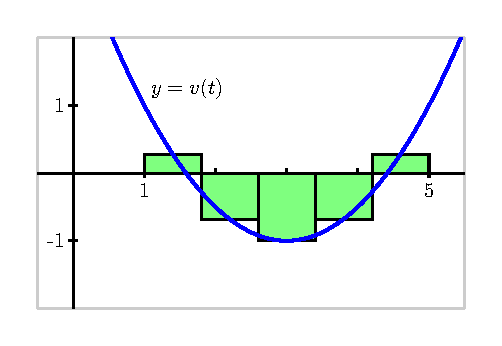
\includegraphics{figures/4_2_Act3Soln.eps}
	\end{center}
	\item Since the net signed area bounded by $v$ on $[1,5]$ represents the total change in position of the object on the interval $[1,5]$, it follows that $M_5$ estimates the total change in position.  Hence, the change in position is approximately $-1.44$ feet.
	\item To estimate the total distance traveled by the object on $[1,5]$, we have to calculate the total area between the curve and the $t$-axis.  Thus,
	$$D \approx \frac{7}{25} \cdot \frac{4}{5} + \frac{17}{25} \cdot \frac{4}{5} + 1 \cdot \frac{4}{5} + \frac{17}{25} \cdot \frac{4}{5} +  \frac{7}{25} \cdot \frac{4}{5} = \frac{292}{125} \approx 2.336.$$
	\item Using appropriate technology, $M_{10} = -1.36$ and $M_{20} = -1.34$.  Further calculations suggest that $M_n \to -\frac{4}{3} = -1.\overline{33}$ as $n \to \infty$, and this number represents the object's total change in position on $[1,5]$.
\ea
\end{activitySolution}
\aftera





 % ACTIVITY

\vspace*{-.5cm}

%-------------
% SUMMARY
%-------------
\begin{summary}
\item A Riemann sum is simply a sum of products of the form $f(x_i^*) \triangle x$ that estimates the area between a positive function and the horizontal axis over a given interval.  If the function is sometimes negative on the interval, the Riemann sum estimates the difference between the areas that lie above the horizontal axis and those that lie below the axis.
\item The three most common types of Riemann sums are left, right, and middle sums, plus we can also work with a more general, random Riemann sum.  The only difference among these sums is the location of the point at which the function is evaluated to determine the height of the rectangle whose area is being computed in the sum.  For a left Riemann sum, we evaluate the function at the left endpoint of each subinterval, while for right and middle sums, we use right endpoints and midpoints, respectively.

\item The left, right, and middle Riemann sums are denoted $L_n$, $R_n$, and $M_n$, with formulas
\[ L_n = f(x_0) \triangle x + f(x_1) \triangle x + \cdots + f(x_{n-1}) \triangle x = \sum_{i = 0}^{n-1} f(x_i) \triangle x, \]
\[ R_n = f(x_1) \triangle x + f(x_2) \triangle x + \cdots + f(x_{n}) \triangle x = \sum_{i = 1}^{n} f(x_i) \triangle x,\]
\[ M_n = f(\overline{x}_1) \triangle x + f(\overline{x}_2) \triangle x + \cdots + f(\overline{x}_{n}) \triangle x = \sum_{i = 1}^{n} f(\overline{x}_i) \triangle x,\]
where $x_0 = a$, $x_i = a + i\triangle x$, and $x_n = b$, using $\triangle x = \frac{b-a}{n}$.  For the midpoint sum, $\overline{x}_{i} = (x_{i-1} + x_i)/2$.
\end{summary} 

\clearpage

%--------------
% EXERCISES
%--------------
\begin{adjustwidth*}{}{-2.25in}
\textbf{{\large Exercises}}
\setlength{\columnsep}{25pt}
\begin{multicols*}{2}
\noindent Terms and Concepts \small
\begin{enumerate}[1)]
\item A fundamental calculus technique is to use \underline{\hskip .5in} to refine approximations to get an exact answer.
\item What is the upper bound in the summation $\ds \sum_{i=7}^{14} (48i-201)$?
\item This section approximates using what geometric shape?
\item T/F: A sum using $R_n$ is an example of a Riemann Sum.
\end{enumerate} 

\noindent {\normalsize Problems} \small

\noindent{\bf In exercises 5--11, write out each term of the summation and compute the sum.}

\bmtwo
\begin{enumerate}[1),resume]
\item $\ds \sum_{i=2}^{4} i^2$
\item $\ds \sum_{i=-1}^{3} (4i-2)$
\item $\ds \sum_{i=-2}^{2} \sin (\pi i/2)$
\item $\ds \sum_{i=1}^{5} \frac1i$
\item $\ds \sum_{i=1}^{6} (-1)^ii$
\item $\ds \sum_{i=1}^{4} \left(\frac{1}{i} - \frac{1}{i+1}\right)$
\item $\ds \sum_{i=0}^{5} (-1)^i\cos (\pi i)$
\end{enumerate}
\emtwo

\noindent{\bf In exercises 12--15, write each sum in summation notation.}

\begin{enumerate}[1),start=12]
\item $3+6+9+12+15$
\item $-1+0+3+8+15+24+35+48+63$
\item $\ds \frac12+\frac23+\frac34+\frac45$
\item $\ds 1-e+e^2-e^3+e^4$
\end{enumerate}

\noindent{\bf In exercises 16--25, evaluate the summation.}

\bmtwo
\begin{enumerate}[1),resume]
\item $\ds \sum_{i=1}^{25} i$
\item $\ds \sum_{i=1}^{10} (3i^2-2i)$
\item $\ds \sum_{i=1}^{15} (2i^3-10)$
\item $\ds \sum_{i=1}^{10} (i^3-3i^2+2i+7)$
\end{enumerate}
\emtwo
\begin{enumerate}[1),start=20]
\item $\ds \sum_{i=1}^{10} (-4i^3+10i^2-7i+11)$
\item $1+4+9+ \ldots +361+400$
\end{enumerate}

\bmtwo
\begin{enumerate}[1),start=22]
\item $\ds \sum_{i=11}^{20} i$
\item $\ds \sum_{i=16}^{25} i^3$
\item $\ds \sum_{i=7}^{12} 4$
\item $\ds \sum_{i=5}^{10} 4i^3$
\end{enumerate}
\emtwo

\columnbreak

\noindent{\bf In exercises 26--31, approximate the area under the given function using the given conditions.}

\begin{enumerate}[1),start=26]
\item $\ds f(x) = x^2$ on $[-3,3]$ with 6 rectangles using $L_n$.
\item $\ds f(x) = 5-x^2$ on $[0,2]$ with 4 rectangles using $M_n$.
\item $\ds f(x) = \sin(x)$ on $[0,\pi]$ with 6 rectangles using $R_n$.
\item $\ds f(x) = 2^x$ on $[0,3]$ with 5 rectangles using $L_n$.
\item $\ds f(x) = \ln(x)$ on $[1,2]$ with 3 rectangles using $M_n$.
\item $\ds f(x) = \frac{1}{x}$ on $[1,9]$ with 4 rectangles using $R_n$.
\end{enumerate}

\noindent{\bf In exercises 32--37, 
\ba
\item find a formula to approximate the area under the given function using $n$ subintervals and the provided rule;
\item evaluate the formula using $n=10, \ 100$, and $1000$; and
\item find the limit of the formula as $n \to \infty$ to compute the exact value of the area under the given function.
\ea}

\begin{enumerate}[1),resume]
\item $\ds f(x) = x^3$ on $[0,1]$ using $R_n$.
\item $\ds f(x) = 3x^2$ on $[-1,1]$ using $L_n$.
\item $\ds f(x) = 3x-1$ on $[-1,3]$ using $M_n$.
\item $\ds f(x) = 2x^2 - 3$ on $[1,4]$ using $L_n$.
\item $\ds f(x) = 5 - x$ on $[-10,10]$ using $R_n$.
\item $\ds f(x) = x^3 - x^2$ on $[0,1]$ using $R_n$.

  \item Consider the function $f(x) = 3x + 4$.
  \ba
  	\item Compute $M_4$ for $y=f(x)$ on the interval $[2,5]$.  Be sure to clearly identify the value of $\triangle x$, as well as the locations of $x_0, x_1, \ldots, x_4$.  Include a careful sketch of the function and the corresponding rectangles being used in the sum.
	\item Use a familiar geometric formula to determine the exact value of the area of the region bounded by $y = f(x)$ and the $x$-axis on $[2,5]$.
	\item Explain why the values you computed in (a) and (b) turn out to be the same.  Will this be true if we use a number different than $n = 4$ and compute $M_n$?  Will $L_4$ or $R_4$ have the same value as the exact area of the region found in (b)?
	\item Describe the collection of functions $g$ for which it will always be the case that $M_n$, regardless of the value of $n$, gives the exact net signed area bounded between the function $g$ and the $x$-axis on the interval $[a,b]$.
  \ea	
\end{enumerate}

%------------------------------------------
% END OF EXERCISES ON FIRST PAGE
%------------------------------------------
\end{multicols*}
\end{adjustwidth*}

\clearpage

\begin{adjustwidth*}{}{-2.25in}
\setlength{\columnsep}{25pt}
\begin{multicols*}{2}\small

\begin{enumerate}[1),start=39]
%ITEM
\item Let $S$ be the sum given by
\begin{align*}
S = & ((1.4)^2 + 1) \cdot 0.4 + ((1.8)^2 + 1) \cdot 0.4 \\
& + ((2.2)^2 + 1) \cdot 0.4 + ((2.6)^2 + 1) \cdot 0.4 \\
& +((3.0)^2 + 1) \cdot 0.4
\end{align*}
  	\ba
		\item Assume that $S$ is a right Riemann sum.  For what function $f$ and what interval $[a,b]$ is $S$ an approximation of the area under $f$ and above the $x$-axis on $[a,b]$?  Why?
		\item How does your answer to (a) change if $S$ is a left Riemann sum?  a middle Riemann sum?
		\item Suppose that $S$ really is a right Riemann sum.  What is geometric quantity does $S$ approximate?
		\item Use sigma notation to write a new sum $R$ that is the right Riemann sum for the same function, but that uses twice as many subintervals as $S$.
	\ea
	
%ITEM
	\item A car traveling along a straight road is braking and its velocity, in ft/sec, is measured at several different points in time, as given in the following table.
\begin{center}
\begin{tabular}{|l|c|c|c|c|c|c|c|}
\hline
seconds, $t$ & $0$ & $0.3$ & $0.6$ & $0.9$ & $1.2$ & $1.5$ & $1.8$ \\
\hline
$v(t)$ & $100$ & $88$ & $74$ & $59$ & $40$ & $19$ & $0$ \\
\hline
\end{tabular}
\end{center}
\ba
	\item Plot the given data on a set of axes with time on the horizontal axis and the velocity on the vertical axis.
	\item Estimate the total distance traveled during the car the time brakes using a middle Riemann sum with 3 subintervals.
	\item Estimate the total distance traveled on $[0,1.8]$ by computing $L_6$, $R_6$, and $\frac{1}{2}(L_6 + R_6)$.
	\item Assuming that $v(t)$ is always decreasing on $[0,1.8]$, what is the maximum possible distance the car traveled before it stopped?  Why?
\ea

%ITEM
	\item The rate at which pollution escapes a scrubbing process at a manufacturing plant increases over time as filters and other technologies become less effective.  For this particular example, assume that the rate of pollution (in tons per week) is given by the function $r$ that is pictured below.
\begin{center}
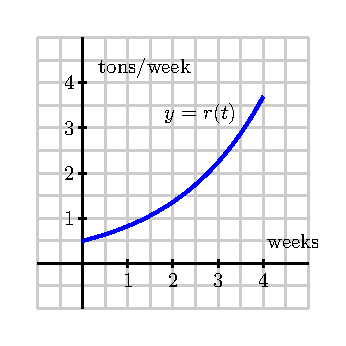
\includegraphics[scale=.75]{figures/4_2_Ez4.eps}
\end{center}
	\ba
		\item Use the graph to estimate the value of $M_4$ on the interval $[0,4]$.
		\item What is the meaning of $M_4$ in terms of the pollution discharged by the plant?
		\item Suppose that $r(t) = 0.5 e^{0.5t}$.  Use this formula for $r$ to compute $L_5$ on $[0,4]$.  
		\item Determine an upper bound on the total amount of pollution that can escape the plant during the pictured four week time period that is accurate within an error of at most one ton of pollution.
	\ea
\end{enumerate}

%---------------------------------------------
% END OF EXERCISES ON SECOND PAGE
%---------------------------------------------
\end{multicols*}
\end{adjustwidth*}

\afterexercises 

\cleardoublepage